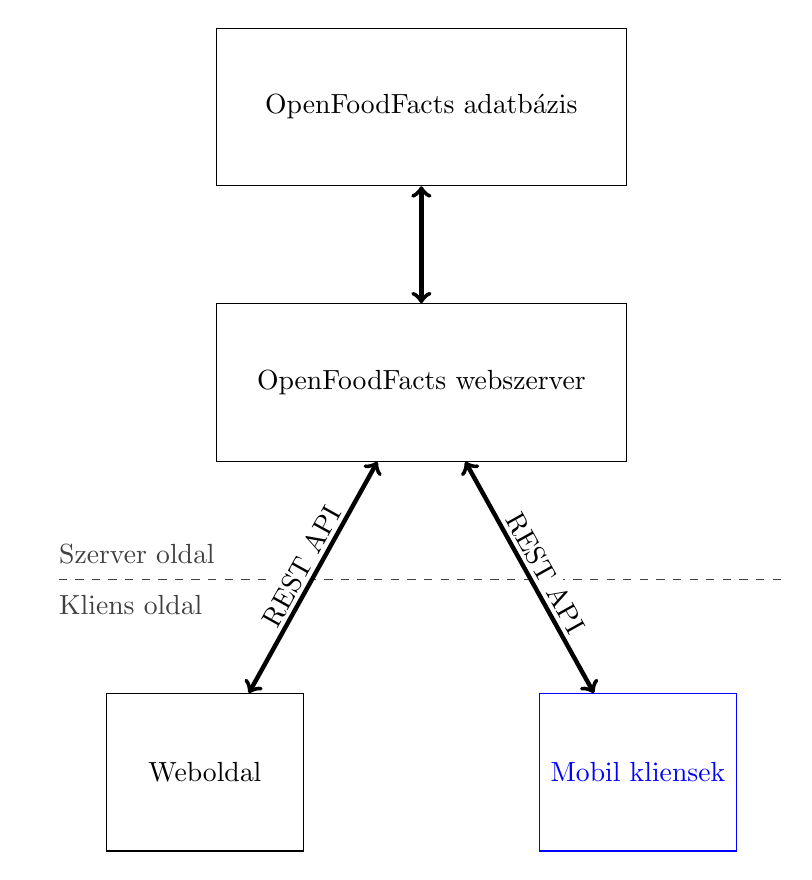
\begin{tikzpicture}[node distance=5cm and 1cm] \label{offarchitektura}
    \begin{scope}
        \node[shape=rectangle,draw,color=black, minimum height=2cm, minimum width=5.2cm] (OFFdb) { OpenFoodFacts adatbázis };
        \node[shape=rectangle, draw, color=black, minimum height=2cm, minimum width=5.2cm, yshift=1.5cm] (OFFwebsrv) [below of = OFFdb] { OpenFoodFacts webszerver };
            \begin{scope}[node distance=7cm]
                \node[shape=rectangle, draw, color=black, minimum height=2cm, minimum width=2.5cm, xshift=2.2cm] (OFFwebsite) [below left of = OFFwebsrv] { Weboldal };
                \node[shape=rectangle, draw, color=blue, minimum height=2cm, minimum width=2.5cm, xshift=-2.2cm] (mobileclients) [below right of = OFFwebsrv] { Mobil kliensek };
            \end{scope}
    \end{scope}
    \begin{scope}
        \path [clip] (-5,-8) rectangle (-1.88,-5) (-1.4,-8) rectangle (1.4,-5) (1.8,-8) rectangle (4.6,-5);
        \draw[darkgray, dashed] ([sloped, xshift=-2cm, yshift=-2.5cm]OFFwebsrv.west) to node [text width=3cm, anchor=west, above, xshift=-3.1cm, yshift=0.075cm] {Szerver oldal} node [text width=3cm, anchor=west, below, xshift=-3.1cm, yshift=-0.075cm] {Kliens oldal} ([sloped, pos=0.5, xshift=2cm, yshift=-2.5cm]OFFwebsrv.east);
    \end{scope}
    \draw[<->, ultra thick] (OFFdb) to node [sloped, pos=0.5, xshift=0.05cm, yshift=0.2cm] {} (OFFwebsrv);
    \draw[<->, ultra thick] (OFFwebsrv) to node [sloped, pos=0.5, xshift=0.05cm, yshift=0.2cm] {REST API} (OFFwebsite);
    \draw[<->, ultra thick] (OFFwebsrv) to node [sloped, pos=0.5, xshift=0.05cm, yshift=0.2cm] {REST API} (mobileclients);
\end{tikzpicture}
